
\section{Doping determination}

Figure~\ref{Fig:ExpH:TSweeps} shows the in-plane resistivity, $\rho(T)$, of the samples in zero fieldtaken in the \ac{VTI} in the Polo magnet. From this plot the mid-transition \Tc values were extracted with error determined from the approximate width of the transition. Results are listed in table~\ref{Table:ExpH:TSweepFitsParams} as well as the normalised \Tc values with $T_c(\textrm{max}) = \unit{36}{\kelvin}$.

\begin{figure}[htbp]
	\begin{center}
		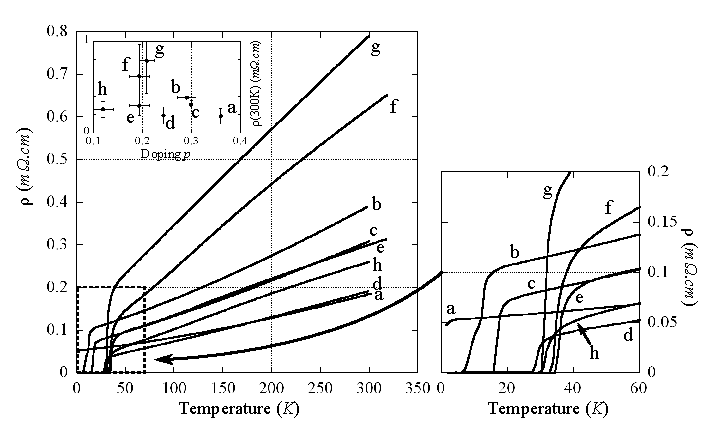
\includegraphics[scale=0.9]{Chapter-HallBSCO/Figures/TSweeps/TSweeps}
		\caption{The in-plane resistivity measured in zero field for each of the samples. From overdoped to underdoped, samples are (a) B00KOD1A, (b) B07KOD2, (c) B16KOD1A, (d) B30KOD3, (e) B32KOP1, (f) B32KOP4, (g) B30KUD3, (h) B28KUD3A. Inset shows a zoomed portion of the curves at the transition temperatures along with continuations of fits to portion of the curve above \Tc in red}
		\label{Fig:ExpH:TSweeps}
	\end{center}
\end{figure}

\begin{figure}[htbp]
    \begin{center}
        \includegraphics[scale=0.9]{Chapter-HallBSCO/Figures/DRhoDtCurves/DRhoDtCurves}
        \caption{$\frac{d\rho(T)}{dT}$ curves for each of the samples taken in zero field. Note the evolution of the $T_{\textrm{coh}}$ gradient in the overdoped samples which give way to the $T^*$ kink in the underdoped samples, B30KUD3 has been repositioned to follow this trend.}
        \label{Fig:ExpH:DRhoDtCurves}
    \end{center}
\end{figure}
The derivatives of the same resistivity curves in figure~\ref{Fig:ExpH:TSweeps} were plotted in figure~\ref{Fig:ExpH:DRhoDtCurves}. Here we can see in the overdoped samples the distinct slope which signifies $T_{\textrm{coh}}$ region. With the exception of B30KUD3, this gradually levels out as doping is reduced until we observe a kink which marks the pseudogap temeprature, $T^*$. By assuming that B30KUD3 is in fact overdoped rather than underdoped --- as the nominal composition would suggest --- then this trend continues right across the range of samples.

Figure~\ref{Fig:ExpH:Dopings} shows the dopings as determined by the three different methods outline din the experimental methods chapter. Clearly the Ando determination bunches the doping values around a much narrower range, whereas the dopings determined by comparing with the \ac{TL2201} \ac{dHvA} data, spread the overdoped values over a wider range.

\begin{figure}[htbp]
    \begin{center}
        \includegraphics[scale=1.1]{Chapter-HallBSCO/Figures/Dopings/Dopings}
        \caption{Doping ditributions for the three different methods. From left to right, B28KUD3a, B30KUD3 (Assume UD), B32KOP1, B32KOP4, B30KUD3 (Assume OD), B30KOD3, B16KOD1a, B07KOD2, B00KOD1a. Broken lines are a guide to the eye. Circled points are B30KUD3 for both the overdoped and underdoped scenarios.}
        \label{Fig:ExpH:Dopings}
    \end{center}
\end{figure}

Further evidence that the B30KUD3 may in fact be an overdoped sample is shown in figure~\ref{Fig:ExpH:Rh300Comparison} where we present our own Hall data at \unit{300}{\kelvin} with comparable data from Konstantinovi\'c \etal~\cite{Konstantinovic2001}.
\begin{figure}[htbp]
    \begin{center}
        \includegraphics[scale=1.0]{Chapter-HallBSCO/Figures/Rh300Comparison/Rh300Comparison}
        \caption{Hall data at \unit{300}{\kelvin} compared with similar data taken from ref~\cite{Konstantinovic2001} using different doping assignments. From left: Tallon relation, Ando relation and scaling to \ac{TL2201} data. Red lines are guides to the eye, circled points are B30KUD3 in the overdoped and underdoped positions.}
        \label{Fig:Rh300Comparison}
    \end{center}
\end{figure}
It is clear that the Ando assigment of dopings is too confined with the data not at all following the respective curve whereas the Tallon relation follows much close the shape of the curve, although, perhaps this is not surprising given that the dopings in the Konstantinovo\'c paper were also assigned using the Tallon relation. However what is most interesting is that of the three methods, the scaling to the \ac{TL2201} \ac{dHvA} data gives the smoothest extrapolation. Also, referring to the circled points, we see that again the data is more consistent if we consider the B30KUD3 to be overdoped rather than underdoped.


